\documentclass{article}

% Language setting
% Replace `english' with e.g. `spanish' to change the document language
\usepackage[english]{babel}

% Set page size and margins
% Replace `letterpaper' with `a4paper' for UK/EU standard size
\usepackage[letterpaper,top=2cm,bottom=2cm,left=3cm,right=3cm,marginparwidth=1.75cm]{geometry}

% Useful packages
\usepackage{amsmath}
\usepackage{graphicx}
\usepackage[colorlinks=true, allcolors=blue]{hyperref}

\begin{document}

\section{The Standard Model}

\subsection{History of the Standard Model, and the Standard Model in plain English}

The study of elementary particle physics traces back to the observation in the 1880s of the production of negative and positive particles, that must be smaller than atoms, in the ionization of gases. The electron was the first subatomic particle to be identified, in 1897 by J. J. Thompson. The fact that atoms consisted mostly of empty space and consisted of a positive charge concentrated at the center, was established in the 1911 ``gold foil" experiment led by Ernest Rutherford. Further experimentation showed that an alpha particle could knock a positively charged particle -- a proton -- out of a nitrogen atom in the air, converting it to carbon. In 1932, a series of experiments established the existence of an electrically neutral particle with about the same mass as the proton -- the neutron. Thus the understanding of particle physics in the 1930s centered around atoms-- known to consist of protons and neutrons, orbited by electrons. 

However, the existence of a fourth particle -- the photon -- was already known, and the picture became increasingly complicated in the 1930s and 1940s with the experiemntal discoveries of the positron, the muon, and the pion. Advances in particle accelerator technology in the 1960s yielded hundreds of particle discoveries. 

\begin{figure}[ht]
    \centering
    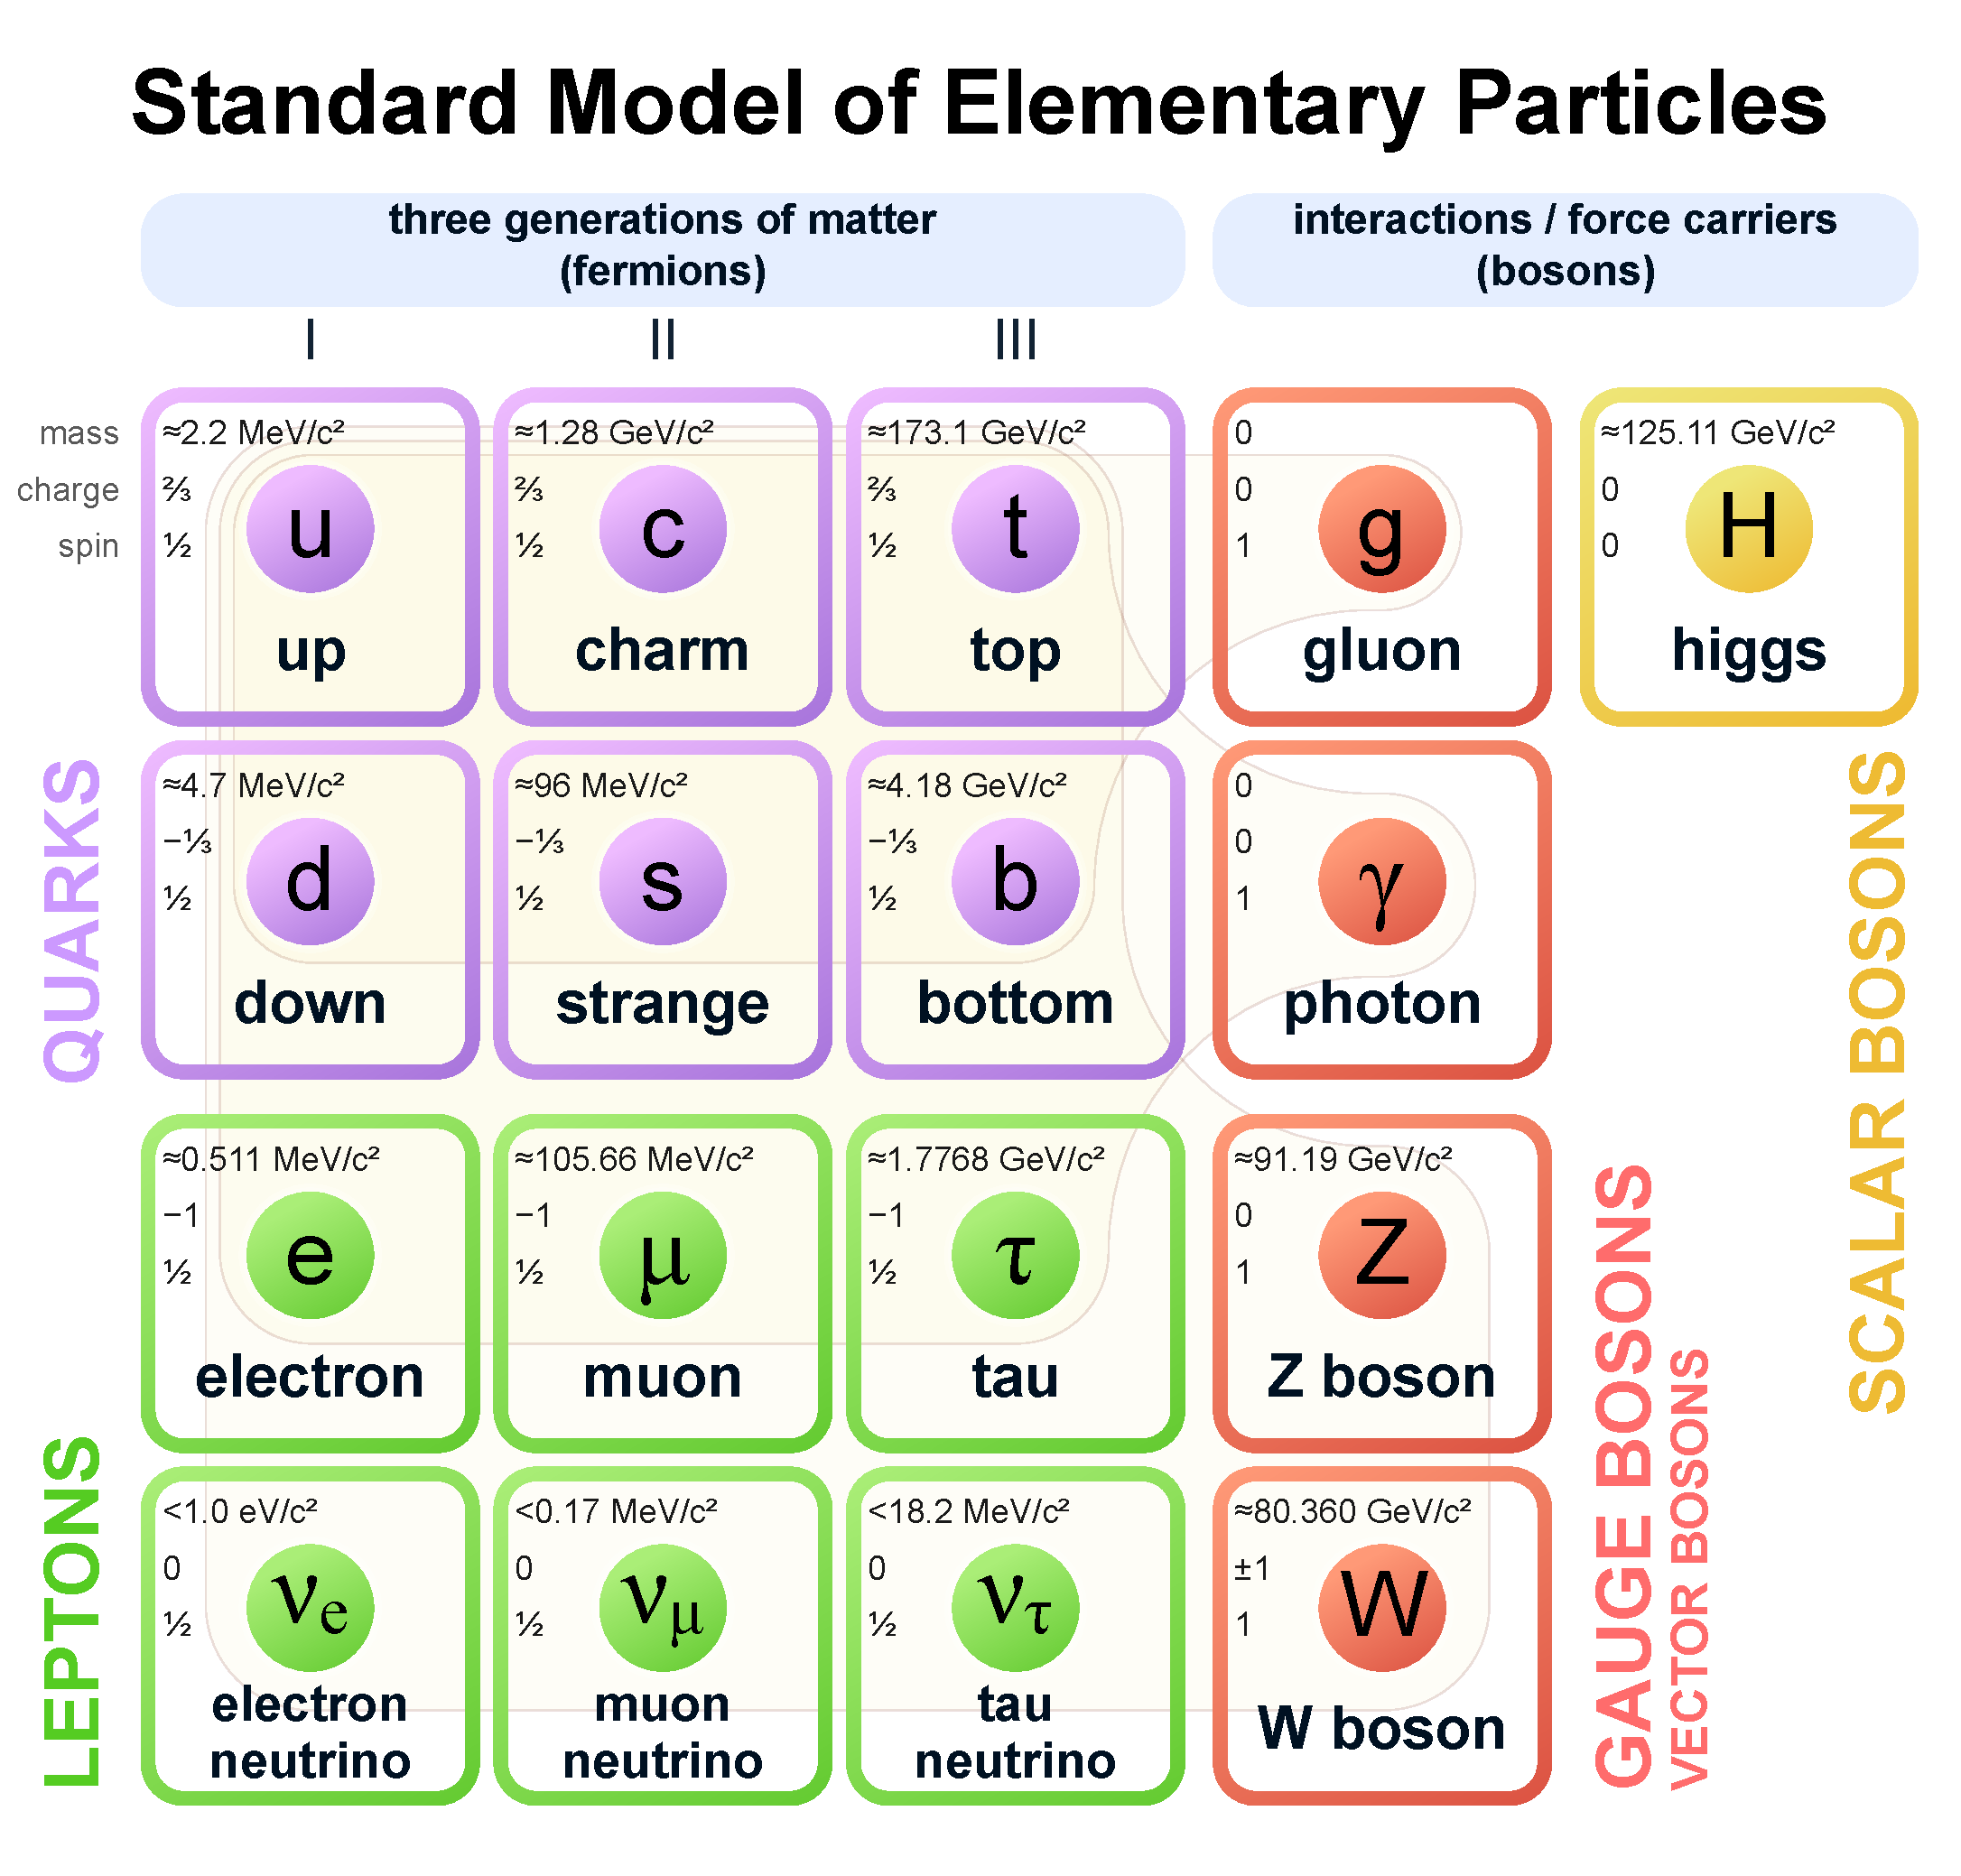
\includegraphics[width=8cm]{figures/Standard_Model_of_Elementary_Particles.pdf}
    \caption{Table of Standard Model particles.}
    \label{fig:intro-standard-model}
\end{figure}



In the absence of a theoretical framework describing these particles, in the 1960s and 1970s physicists and mathematicians produced a theoretical framework called the \textbf{Standard Model (SM)} that could describe and encompass these fundamental particles and the forces that govern their interactions. The application of a mathematical theorem derived by Emmy Noether in 1918, which states that every continuous symmetry of the action of a physical system with conservative forces, has a corresponding conservation law, allowed the grouping of seventeen fundamental particles, shown in Fig. \ref{fig:intro-standard-model}.

The Standard Model groups these seventeen fundamental particles into fermions and bosons. \textbf{Fermions} consist of quarks and leptons. Quarks and leptons are grouped into three generations of matter. For example, the familiar electron falls into the first generation of leptons. The second and third generation counterparts of the electron are the muon and the tau, and are over 200 and 30,000 times heavier than the electron respectively. \textbf{Bosons} are force carriers -- in the formulation of the Standard Model, the interaction of fermions with bosons, corresponds to fundamental forces. The Standard Model describes the electromagnetic force, the strong nuclear force, and the weak nuclear force.


\subsection{The mathematics of the Standard Model}

Each force in the Standard Model is associated to a Lie group. A Lie group a type of group (a set of operations) that is also a differentiable manifold- in other words, Lie groups can be studied with differential calculus. An example of a Lie group is the rotation matrices, denoted $SO(2, \mathcal{R})$. With the rotation angle $\phi$, this group can be parametrized as: $$SO(2, \mathcal{R}) = \begin{pmatrix} \cos\phi & -\sin\phi \\ \sin\phi & \cos\phi \end{pmatrix}, \,\, \phi \in \mathcal{R}/2\pi\mathcal{Z}$$

The Standard Model is built around the group $$G = U(1) \times SU(2) \times SU(3).$$ $SU(3)$ is associated to the strong force; $SU(2)$ is associated to the weak force; and $U(1)$ is not electromagnetism, but rather the weak force. Electromagnetism arises from the terms $SU(2) \times U(1)$. 

In the Standard Model, forces are associated with the gauge bosons, which are massless spin-1 particles. These forces are governed by \textbf{gauge invariance}. The most familiar example of gauge invariance is in electromagnetism, where the fundamental field is the gauge potential 4-vector $A_\mu(x)$. Not all components of this field are physical. Any two choice of gauge potentials related by a transformation of the form \begin{equation} A_\mu \rightarrow A_\mu + \partial_\mu \alpha \label{eqn:gauge_symmetry}\end{equation} for any function $\alpha(x)$, describe the same physical configuration. This transformation in Eqn. \ref{eqn:gauge_symmetry} is often referred to as a \textbf{gauge symmetry}, but as Tong puts it, may be more aptly called \textbf{gauge redundancy}.

The meaning of  function $\alpha(x)$ func

For the gauge bosons of the Standard Model, the fields are labeled $A_\mu^{A}$. Again, not all of the information in $A_\mu$ is physical, and any field configurations related by a gauge transformation are equivalent. However, the gauge transformation is more complex than that of \ref{eqn:gauge_symmetry}.

% https://www.damtp.cam.ac.uk/user/tong/sm/standardmodel1.pdf

\section{Sources}

    \begin{itemize}
        \item \texttt{https://www.space.com/standard-model-physics}
        \item \texttt{https://www.iop.org/explore-physics/big-ideas-physics/standard-model}
        \item Wikipedia
        \item \texttt{https://www.damtp.cam.ac.uk/user/tong/sm/standardmodel1.pdf}
    \end{itemize}

\end{document}